\section{Evaluation}
\label{sec:evaluation}
DCG-UPUP-Away is evaluated in two experiments.
First, a simulated turtlebot within randomly generated simulated environments is given a series of user-generated natural language commands.
Second, a physical turtlebot is given specific commands in a laboratory environment in order to demonstrate novel behaviors enabled by DCG-UPUP-Away.
Both experiments assume a perfect object recognizer that translates raw sensor data into a world model $\Upsilon$ that may be used by DCG-UPUP-Away, as well as an initial set of hand-labeled training examples for training the LLM to ground cubes, spheres, and cylinders.\\
\subsection{Experimental Setup}
\indent The simulated testing environments are randomly generated in Gazebo.
10 worlds are created, and each is populated with a random collection of objects in randomized locations.
There are 8 possible object types (including cubes, spheres, and cylinders) in 3 possible colors, for a total of 24 objects.
Each object has a 15\% chance of being added to a given map.\\
\indent After generating the 10 maps, screenshots of world with a single object highlighted are uploaded to Amazon Mechanical Turk.
For each image, users were instructed to write a command ``for approaching the highlighted object.''
These image-command pairs are then saved for evaluating whether a robot, when placed in the corresponding simulated world and given the natural language command, successfully approaches the correct object.
An example screenshot, with an annotation supplied by a user, is shown in Figure~\ref{fig:amt}.\\
\begin{figure}[h]
	\centering
    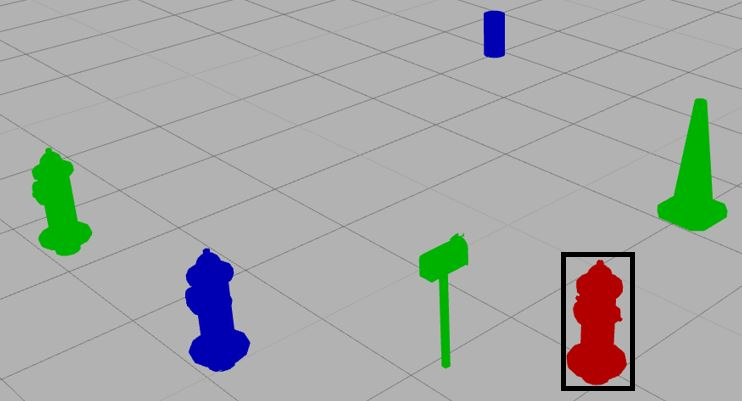
\includegraphics[width=8.5cm]{amt}
	\caption{A simulated world with a highlighted object presented on Amazon Mechanical Turk, labeled by a user as ``Move to the red fire hydrant.''}
	\label{fig:amt}
\end{figure}
The metrics we consider are the grounding accuracy (how likely DCG-UPUP-Away is to correctly ground a phrase) and the number of known symbols.

\subsection{Grounding Accuracy}
here I show the grounding accuracy (as well as how need hypothetical groundings)

I plot the grounding accuracy.
\begin{figure}[h]
\centering
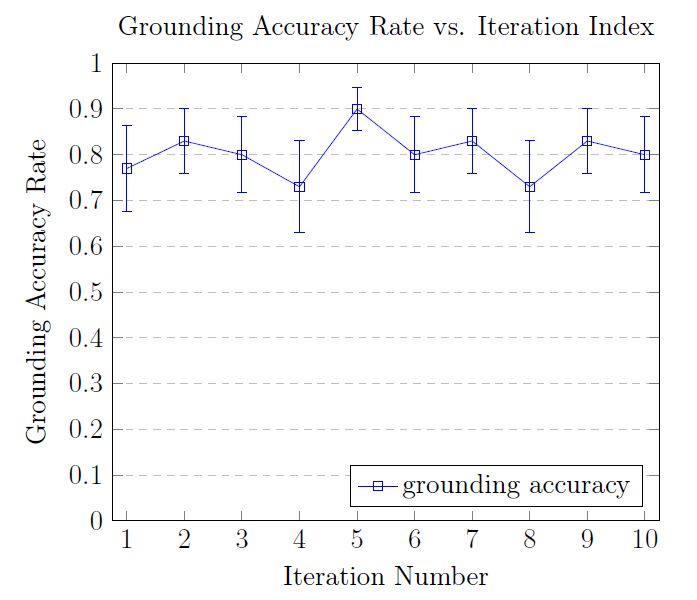
\includegraphics[width=8.5cm]{g_acc}
\caption{this is the overall grounding accuracy}
\label{fig:g_acc}
\end{figure}

Here I split up the success cases, normalized by the overall accuracy rate, for known, unknown, and learned.
\begin{figure}[h]
\centering
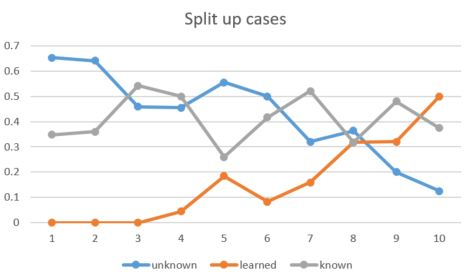
\includegraphics[width=8.5cm]{learning}
\caption{this is split up (must replot well)}
\label{fig:g_acc}
\end{figure}


\subsection{Learned Symbols}
here I show how DCG-UPUP-Away learns symbols
\begin{figure}[h]
\centering
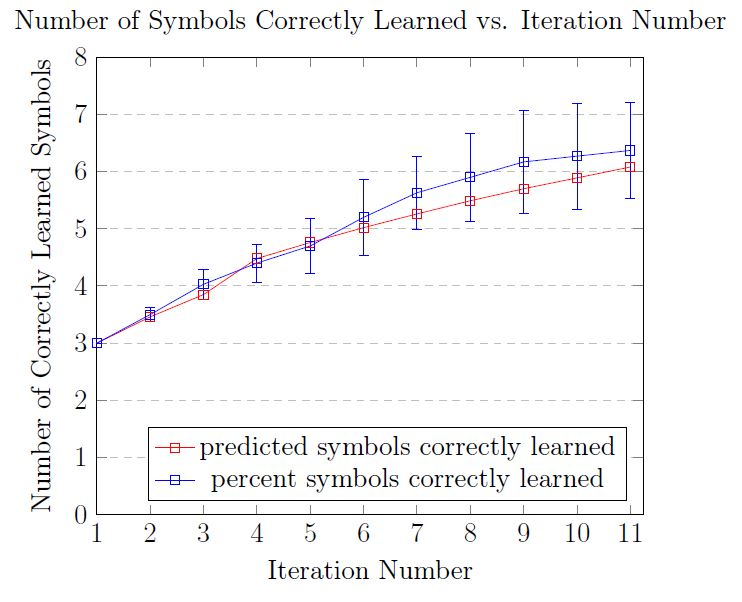
\includegraphics[width=8.5cm]{symbols_corr}
\caption{this is how we show that we learn symbols. I will update this label (and caption) of this figure}
\label{fig:g_acc}
\end{figure}

\subsection{Hardware Demonstration}
Outside the simulation environment, DCG-UPUP-Away was tested on a physical turtlebot in a laboratory setting.
The turtlebot was placed facing a cylinder (known) and a cone (unknown).
In addition, a cube (known) and a crate (unknown) were located behind the turtlebot.
All objects were labeled with AR-track tags, which, in conjunction with (cite AR track package) was used in order to generate the world model $\Upsilon$ from a kinect mounted on the turtlebot.\\
%I'd like to add a footnote saying that I have videos of these demos
\indent Four natural language commands were used to demonstrate the full range of abilities of DCG-UPUP-Away.
First, the turtlebot was given the command ``move towards the cube.''
The turtlebot successfully drove to the cube, demonstrating a correct grounding to a known, perceived object.\\
\indent Second, the turtlebot was given the command ``move towards the cone.''
The turtlebot drove to the cone, demonstrating that it perceived the cone as unknown, recognized the phrase ``cone'' as unknown, and grounded the unknown phrase to the unknown object.
Thus, a command was correctly grounded to an unknown, perceived object.\\
\indent Third, the turtlebot was given the command ``move towards the cube.''
The turtlebot rotated in place until the cube came in view, and then approached the cube.
In other words, the command was first grounded to a known, hypothesized object and then, once then cube was perceived, to a known, perceived object.\\
\indent Fourth, the turtlebot was given the command ``move towards the crate.''
Once again, the turtlebot rotated in place, this time until it saw the crate, whereupon it drove to the crate.
This demonstrates two important behaviors: 1) the turtlebot must have learned what a cone was, otherwise the unknown phrase (``crate'') would have been grounded to the cone and 2) the turtlebot grounded the command to an unknown, hypothesized object until the crate was perceived.
The execution of this last command, including images of the physical behavior of the turtlebot as well as the model used for grounding, is shown in Figure~\ref{fig:hardware_demo}.

\begin{figure}[ht]
\centering
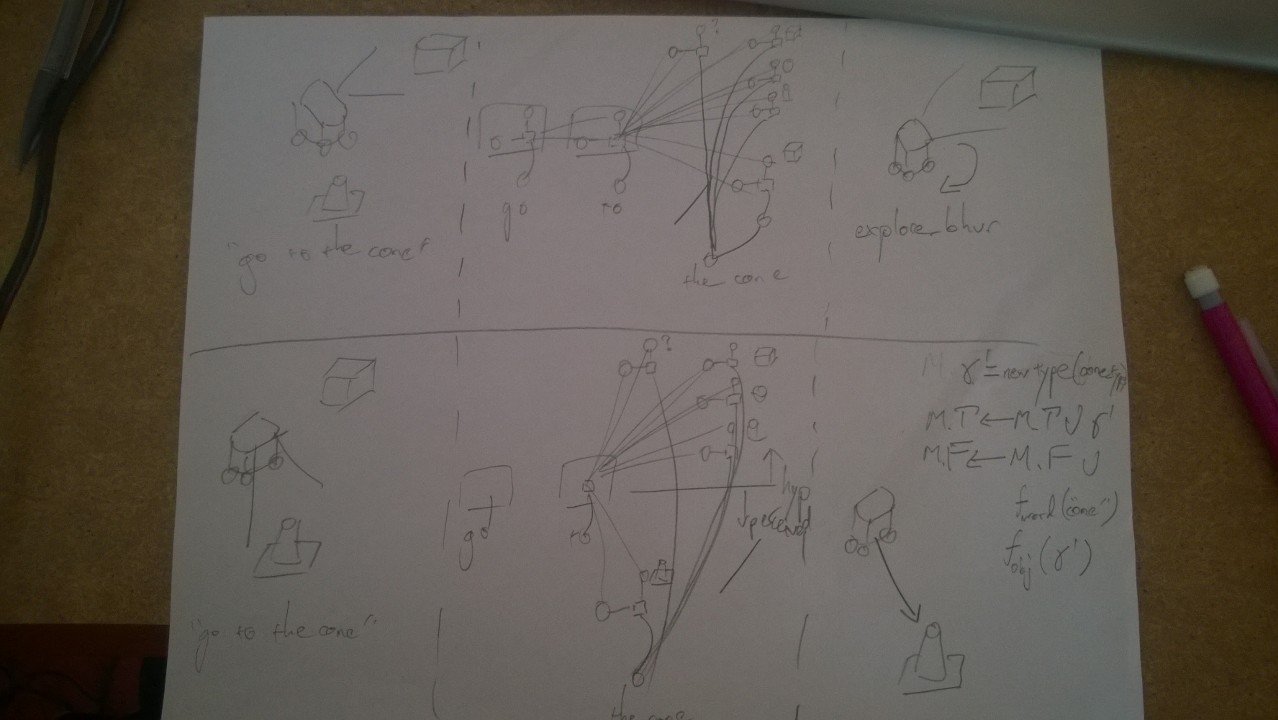
\includegraphics[width=8.5cm]{hardware_sketch}
\caption{this is a sketch of the 6 subfigures that demonstrate hypothesized groundings on hardware and in the model, and shows how it learns. I'd like this to go across the top of the page.}
\label{fig:hardware_demo}
\end{figure}

\subsection{Limitations}
here I saw what the limitations are